\documentclass[1p]{elsarticle_modified}
%\bibliographystyle{elsarticle-num}

%\usepackage[colorlinks]{hyperref}
%\usepackage{abbrmath_seonhwa} %\Abb, \Ascr, \Acal ,\Abf, \Afrak
\usepackage{amsfonts}
\usepackage{amssymb}
\usepackage{amsmath}
\usepackage{amsthm}
\usepackage{scalefnt}
\usepackage{amsbsy}
\usepackage{kotex}
\usepackage{caption}
\usepackage{subfig}
\usepackage{color}
\usepackage{graphicx}
\usepackage{xcolor} %% white, black, red, green, blue, cyan, magenta, yellow
\usepackage{float}
\usepackage{setspace}
\usepackage{hyperref}

\usepackage{tikz}
\usetikzlibrary{arrows}

\usepackage{multirow}
\usepackage{array} % fixed length table
\usepackage{hhline}

%%%%%%%%%%%%%%%%%%%%%
\makeatletter
\renewcommand*\env@matrix[1][\arraystretch]{%
	\edef\arraystretch{#1}%
	\hskip -\arraycolsep
	\let\@ifnextchar\new@ifnextchar
	\array{*\c@MaxMatrixCols c}}
\makeatother %https://tex.stackexchange.com/questions/14071/how-can-i-increase-the-line-spacing-in-a-matrix
%%%%%%%%%%%%%%%

\usepackage[normalem]{ulem}

\newcommand{\msout}[1]{\ifmmode\text{\sout{\ensuremath{#1}}}\else\sout{#1}\fi}
%SOURCE: \msout is \stkout macro in https://tex.stackexchange.com/questions/20609/strikeout-in-math-mode

\newcommand{\cancel}[1]{
	\ifmmode
	{\color{red}\msout{#1}}
	\else
	{\color{red}\sout{#1}}
	\fi
}

\newcommand{\add}[1]{
	{\color{blue}\uwave{#1}}
}

\newcommand{\replace}[2]{
	\ifmmode
	{\color{red}\msout{#1}}{\color{blue}\uwave{#2}}
	\else
	{\color{red}\sout{#1}}{\color{blue}\uwave{#2}}
	\fi
}

\newcommand{\Sol}{\mathcal{S}} %segment
\newcommand{\D}{D} %diagram
\newcommand{\A}{\mathcal{A}} %arc


%%%%%%%%%%%%%%%%%%%%%%%%%%%%%5 test

\def\sl{\operatorname{\textup{SL}}(2,\Cbb)}
\def\psl{\operatorname{\textup{PSL}}(2,\Cbb)}
\def\quan{\mkern 1mu \triangleright \mkern 1mu}

\theoremstyle{definition}
\newtheorem{thm}{Theorem}[section]
\newtheorem{prop}[thm]{Proposition}
\newtheorem{lem}[thm]{Lemma}
\newtheorem{ques}[thm]{Question}
\newtheorem{cor}[thm]{Corollary}
\newtheorem{defn}[thm]{Definition}
\newtheorem{exam}[thm]{Example}
\newtheorem{rmk}[thm]{Remark}
\newtheorem{alg}[thm]{Algorithm}

\newcommand{\I}{\sqrt{-1}}
\begin{document}

%\begin{frontmatter}
%
%\title{Boundary parabolic representations of knots up to 8 crossings}
%
%%% Group authors per affiliation:
%\author{Yunhi Cho} 
%\address{Department of Mathematics, University of Seoul, Seoul, Korea}
%\ead{yhcho@uos.ac.kr}
%
%
%\author{Seonhwa Kim} %\fnref{s_kim}}
%\address{Center for Geometry and Physics, Institute for Basic Science, Pohang, 37673, Korea}
%\ead{ryeona17@ibs.re.kr}
%
%\author{Hyuk Kim}
%\address{Department of Mathematical Sciences, Seoul National University, Seoul 08826, Korea}
%\ead{hyukkim@snu.ac.kr}
%
%\author{Seokbeom Yoon}
%\address{Department of Mathematical Sciences, Seoul National University, Seoul, 08826,  Korea}
%\ead{sbyoon15@snu.ac.kr}
%
%\begin{abstract}
%We find all boundary parabolic representation of knots up to 8 crossings.
%
%\end{abstract}
%\begin{keyword}
%    \MSC[2010] 57M25 
%\end{keyword}
%
%\end{frontmatter}

%\linenumbers
%\tableofcontents
%
\newcommand\colored[1]{\textcolor{white}{\rule[-0.35ex]{0.8em}{1.4ex}}\kern-0.8em\color{red} #1}%
%\newcommand\colored[1]{\textcolor{white}{ #1}\kern-2.17ex	\textcolor{white}{ #1}\kern-1.81ex	\textcolor{white}{ #1}\kern-2.15ex\color{red}#1	}

{\Large $\underline{11n_{143}~(K11n_{143})}$}

\setlength{\tabcolsep}{10pt}
\renewcommand{\arraystretch}{1.6}
\vspace{1cm}\begin{tabular}{m{100pt}>{\centering\arraybackslash}m{274pt}}
\multirow{5}{120pt}{
	\centering
	\includegraphics[width=112pt]{../../../GIT/diagram.site/Diagrams/png/759_11n_143.png}\\
\ \ \ A knot diagram\footnotemark}&
\allowdisplaybreaks
\textbf{Linearized knot diagam} \\
\cline{2-2}
 &
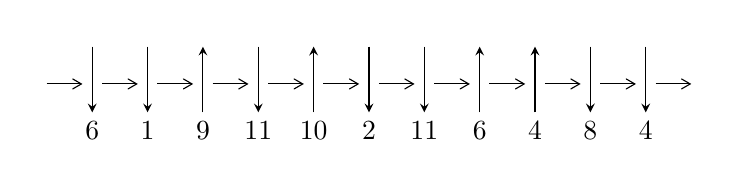
\begin{tikzpicture}[x=20pt, y=17pt]
	% nodes
	\node (C0) at (0, 0) {};
	\node (C1) at (1, 0) {};
	\node (C1U) at (1, +1) {};
	\node (C1D) at (1, -1) {6};

	\node (C2) at (2, 0) {};
	\node (C2U) at (2, +1) {};
	\node (C2D) at (2, -1) {1};

	\node (C3) at (3, 0) {};
	\node (C3U) at (3, +1) {};
	\node (C3D) at (3, -1) {9};

	\node (C4) at (4, 0) {};
	\node (C4U) at (4, +1) {};
	\node (C4D) at (4, -1) {11};

	\node (C5) at (5, 0) {};
	\node (C5U) at (5, +1) {};
	\node (C5D) at (5, -1) {10};

	\node (C6) at (6, 0) {};
	\node (C6U) at (6, +1) {};
	\node (C6D) at (6, -1) {2};

	\node (C7) at (7, 0) {};
	\node (C7U) at (7, +1) {};
	\node (C7D) at (7, -1) {11};

	\node (C8) at (8, 0) {};
	\node (C8U) at (8, +1) {};
	\node (C8D) at (8, -1) {6};

	\node (C9) at (9, 0) {};
	\node (C9U) at (9, +1) {};
	\node (C9D) at (9, -1) {4};

	\node (C10) at (10, 0) {};
	\node (C10U) at (10, +1) {};
	\node (C10D) at (10, -1) {8};

	\node (C11) at (11, 0) {};
	\node (C11U) at (11, +1) {};
	\node (C11D) at (11, -1) {4};
	\node (C12) at (12, 0) {};

	% arrows
	\draw[->,>={angle 60}]
	(C0) edge (C1) (C1) edge (C2) (C2) edge (C3) (C3) edge (C4) (C4) edge (C5) (C5) edge (C6) (C6) edge (C7) (C7) edge (C8) (C8) edge (C9) (C9) edge (C10) (C10) edge (C11) (C11) edge (C12) ;	\draw[->,>=stealth]
	(C1U) edge (C1D) (C2U) edge (C2D) (C3D) edge (C3U) (C4U) edge (C4D) (C5D) edge (C5U) (C6U) edge (C6D) (C7U) edge (C7D) (C8D) edge (C8U) (C9D) edge (C9U) (C10U) edge (C10D) (C11U) edge (C11D) ;
	\end{tikzpicture} \\
\hhline{~~} \\& 
\textbf{Solving Sequence} \\ \cline{2-2} 
 &
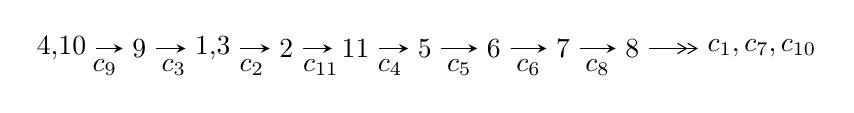
\begin{tikzpicture}[x=25pt, y=7pt]
	% node
	\node (A0) at (-1/8, 0) {4,10};
	\node (A1) at (1, 0) {9};
	\node (A2) at (33/16, 0) {1,3};
	\node (A3) at (25/8, 0) {2};
	\node (A4) at (33/8, 0) {11};
	\node (A5) at (41/8, 0) {5};
	\node (A6) at (49/8, 0) {6};
	\node (A7) at (57/8, 0) {7};
	\node (A8) at (65/8, 0) {8};
	\node (C1) at (1/2, -1) {$c_{9}$};
	\node (C2) at (3/2, -1) {$c_{3}$};
	\node (C3) at (21/8, -1) {$c_{2}$};
	\node (C4) at (29/8, -1) {$c_{11}$};
	\node (C5) at (37/8, -1) {$c_{4}$};
	\node (C6) at (45/8, -1) {$c_{5}$};
	\node (C7) at (53/8, -1) {$c_{6}$};
	\node (C8) at (61/8, -1) {$c_{8}$};
	\node (A9) at (10, 0) {$c_{1},c_{7},c_{10}$};

	% edge
	\draw[->,>=stealth]	
	(A0) edge (A1) (A1) edge (A2) (A2) edge (A3) (A3) edge (A4) (A4) edge (A5) (A5) edge (A6) (A6) edge (A7) (A7) edge (A8) ;
	\draw[->>,>={angle 60}]	
	(A8) edge (A9);
\end{tikzpicture} \\ 

\end{tabular} \\

\footnotetext{
The image of knot diagram is generated by the software ``\textbf{Draw programme}" developed by Andrew Bartholomew(\url{http://www.layer8.co.uk/maths/draw/index.htm\#Running-draw}), where we modified some parts for our purpose(\url{https://github.com/CATsTAILs/LinksPainter}).
}\phantom \\ \newline 
\centering \textbf{Ideals for irreducible components\footnotemark of $X_{\text{par}}$} 
 
\begin{align*}
I^u_{1}&=\langle 
27169327131 u^{12}-4728521972 u^{11}+\cdots+163375109309 b+102043710068,\\
\phantom{I^u_{1}}&\phantom{= \langle  }46748483168 u^{12}-1185808565 u^{11}+\cdots+163375109309 a-246903703505,\\
\phantom{I^u_{1}}&\phantom{= \langle  }u^{13}- u^{12}-16 u^{11}+13 u^{10}+93 u^9-90 u^8+85 u^7-4 u^6+11 u^5-20 u^4+2 u^2+u-1\rangle \\
I^u_{2}&=\langle 
3 u^8-5 u^6- u^5-7 u^4-6 u^3+b-3 u+2,\;-2 u^8+u^7+3 u^6- u^5+4 u^4+3 u^3- u^2+a+2 u-1,\\
\phantom{I^u_{2}}&\phantom{= \langle  }u^9- u^7-3 u^5-3 u^4-2 u^3-3 u^2- u-1\rangle \\
\\
\end{align*}
\raggedright * 2 irreducible components of $\dim_{\mathbb{C}}=0$, with total 22 representations.\\
\footnotetext{All coefficients of polynomials are rational numbers. But the coefficients are sometimes approximated in decimal forms when there is not enough margin.}
\newpage
\renewcommand{\arraystretch}{1}
\centering \section*{I. $I^u_{1}= \langle 2.72\times10^{10} u^{12}-4.73\times10^{9} u^{11}+\cdots+1.63\times10^{11} b+1.02\times10^{11},\;4.67\times10^{10} u^{12}-1.19\times10^{9} u^{11}+\cdots+1.63\times10^{11} a-2.47\times10^{11},\;u^{13}- u^{12}+\cdots+u-1 \rangle$}
\flushleft \textbf{(i) Arc colorings}\\
\begin{tabular}{m{7pt} m{180pt} m{7pt} m{180pt} }
\flushright $a_{4}=$&$\begin{pmatrix}0\\u\end{pmatrix}$ \\
\flushright $a_{10}=$&$\begin{pmatrix}1\\0\end{pmatrix}$ \\
\flushright $a_{9}=$&$\begin{pmatrix}1\\u^2\end{pmatrix}$ \\
\flushright $a_{1}=$&$\begin{pmatrix}-0.286142 u^{12}+0.00725820 u^{11}+\cdots+0.326465 u+1.51127\\-0.166300 u^{12}+0.0289427 u^{11}+\cdots-0.0380012 u-0.624598\end{pmatrix}$ \\
\flushright $a_{3}=$&$\begin{pmatrix}- u\\- u^3+u\end{pmatrix}$ \\
\flushright $a_{2}=$&$\begin{pmatrix}-1.45178 u^{12}+1.36239 u^{11}+\cdots-1.27398 u-1.38184\\-0.0325056 u^{12}+0.182051 u^{11}+\cdots-1.79766 u-0.0596779\end{pmatrix}$ \\
\flushright $a_{11}=$&$\begin{pmatrix}-0.286142 u^{12}+0.00725820 u^{11}+\cdots+0.326465 u+1.51127\\-0.0919107 u^{12}+0.0169286 u^{11}+\cdots-0.0307430 u-0.345714\end{pmatrix}$ \\
\flushright $a_{5}=$&$\begin{pmatrix}1.39226 u^{12}-1.21256 u^{11}+\cdots-1.08841 u+1.29245\\0.0595160 u^{12}-0.149831 u^{11}+\cdots+2.36239 u+0.0893943\end{pmatrix}$ \\
\flushright $a_{6}=$&$\begin{pmatrix}1.45178 u^{12}-1.36239 u^{11}+\cdots+1.27398 u+1.38184\\0.0595160 u^{12}-0.149831 u^{11}+\cdots+2.36239 u+0.0893943\end{pmatrix}$ \\
\flushright $a_{7}=$&$\begin{pmatrix}0.286142 u^{12}-0.00725820 u^{11}+\cdots-0.326465 u-1.51127\\0.0289310 u^{12}+0.00713908 u^{11}+\cdots+0.000702000 u+0.287036\end{pmatrix}$ \\
\flushright $a_{8}=$&$\begin{pmatrix}0.0893943 u^{12}-0.0298782 u^{11}+\cdots-0.0699394 u+2.45178\\-0.0903148 u^{12}+0.0234848 u^{11}+\cdots+0.0298782 u+0.0595160\end{pmatrix}$\\ \flushright $a_{8}=$&$\begin{pmatrix}0.0893943 u^{12}-0.0298782 u^{11}+\cdots-0.0699394 u+2.45178\\-0.0903148 u^{12}+0.0234848 u^{11}+\cdots+0.0298782 u+0.0595160\end{pmatrix}$\\&\end{tabular}
\flushleft \textbf{(ii) Obstruction class $= -1$}\\~\\
\flushleft \textbf{(iii) Cusp Shapes $= -\frac{425649841644}{163375109309} u^{12}+\frac{257561868150}{163375109309} u^{11}+\cdots+\frac{821280596494}{163375109309} u-\frac{283918679660}{163375109309}$}\\~\\
\newpage\renewcommand{\arraystretch}{1}
\flushleft \textbf{(iv) u-Polynomials at the component}\newline \\
\begin{tabular}{m{50pt}|m{274pt}}
Crossings & \hspace{64pt}u-Polynomials at each crossing \\
\hline $$\begin{aligned}c_{1},c_{6}\end{aligned}$$&$\begin{aligned}
&u^{13}-11 u^{12}+\cdots-48 u+16
\end{aligned}$\\
\hline $$\begin{aligned}c_{2}\end{aligned}$$&$\begin{aligned}
&u^{13}+7 u^{12}+\cdots-640 u+256
\end{aligned}$\\
\hline $$\begin{aligned}c_{3},c_{8},c_{9}\end{aligned}$$&$\begin{aligned}
&u^{13}+u^{12}+\cdots+u+1
\end{aligned}$\\
\hline $$\begin{aligned}c_{4},c_{11}\end{aligned}$$&$\begin{aligned}
&u^{13}-3 u^{12}+\cdots-2 u+1
\end{aligned}$\\
\hline $$\begin{aligned}c_{5}\end{aligned}$$&$\begin{aligned}
&u^{13}-14 u^{11}+\cdots+13 u+6
\end{aligned}$\\
\hline $$\begin{aligned}c_{7},c_{10}\end{aligned}$$&$\begin{aligned}
&u^{13}-3 u^{12}+\cdots+3 u-1
\end{aligned}$\\
\hline
\end{tabular}\\~\\
\newpage\renewcommand{\arraystretch}{1}
\flushleft \textbf{(v) Riley Polynomials at the component}\newline \\
\begin{tabular}{m{50pt}|m{274pt}}
Crossings & \hspace{64pt}Riley Polynomials at each crossing \\
\hline $$\begin{aligned}c_{1},c_{6}\end{aligned}$$&$\begin{aligned}
&y^{13}-7 y^{12}+\cdots-640 y-256
\end{aligned}$\\
\hline $$\begin{aligned}c_{2}\end{aligned}$$&$\begin{aligned}
&y^{13}+69 y^{12}+\cdots-106496 y-65536
\end{aligned}$\\
\hline $$\begin{aligned}c_{3},c_{8},c_{9}\end{aligned}$$&$\begin{aligned}
&y^{13}-33 y^{12}+\cdots+5 y-1
\end{aligned}$\\
\hline $$\begin{aligned}c_{4},c_{11}\end{aligned}$$&$\begin{aligned}
&y^{13}+27 y^{12}+\cdots-34 y-1
\end{aligned}$\\
\hline $$\begin{aligned}c_{5}\end{aligned}$$&$\begin{aligned}
&y^{13}-28 y^{12}+\cdots-83 y-36
\end{aligned}$\\
\hline $$\begin{aligned}c_{7},c_{10}\end{aligned}$$&$\begin{aligned}
&y^{13}+y^{12}+\cdots- y-1
\end{aligned}$\\
\hline
\end{tabular}\\~\\
\newpage\flushleft \textbf{(vi) Complex Volumes and Cusp Shapes}
$$\begin{array}{c|c|c}  
\text{Solutions to }I^u_{1}& \I (\text{vol} + \sqrt{-1}CS) & \text{Cusp shape}\\
 \hline 
\begin{aligned}
u &= \phantom{-}0.444507 + 0.873153 I \\
a &= \phantom{-}0.145964 + 0.210434 I \\
b &= -0.10255 - 2.20008 I\end{aligned}
 & -5.13656 + 3.94627 I & \phantom{-}0.021726 + 1.151779 I \\ \hline\begin{aligned}
u &= \phantom{-}0.444507 - 0.873153 I \\
a &= \phantom{-}0.145964 - 0.210434 I \\
b &= -0.10255 + 2.20008 I\end{aligned}
 & -5.13656 - 3.94627 I & \phantom{-}0.021726 - 1.151779 I \\ \hline\begin{aligned}
u &= -0.278059 + 0.532845 I \\
a &= \phantom{-}0.482522 - 0.330538 I \\
b &= -0.243913 + 0.386628 I\end{aligned}
 & -0.112278 - 1.172770 I & -1.56848 + 5.39486 I \\ \hline\begin{aligned}
u &= -0.278059 - 0.532845 I \\
a &= \phantom{-}0.482522 + 0.330538 I \\
b &= -0.243913 - 0.386628 I\end{aligned}
 & -0.112278 + 1.172770 I & -1.56848 - 5.39486 I \\ \hline\begin{aligned}
u &= \phantom{-}0.581027\phantom{ +0.000000I} \\
a &= \phantom{-}1.33008\phantom{ +0.000000I} \\
b &= \phantom{-}0.743719\phantom{ +0.000000I}\end{aligned}
 & -1.77301\phantom{ +0.000000I} & -4.59260\phantom{ +0.000000I} \\ \hline\begin{aligned}
u &= -0.395821 + 0.255747 I \\
a &= \phantom{-}1.63033 - 1.89256 I \\
b &= -0.681021 - 0.928853 I\end{aligned}
 & \phantom{-}3.39477 - 1.45394 I & \phantom{-}0.239284 + 0.384387 I \\ \hline\begin{aligned}
u &= -0.395821 - 0.255747 I \\
a &= \phantom{-}1.63033 + 1.89256 I \\
b &= -0.681021 + 0.928853 I\end{aligned}
 & \phantom{-}3.39477 + 1.45394 I & \phantom{-}0.239284 - 0.384387 I \\ \hline\begin{aligned}
u &= \phantom{-}0.364118 + 0.280685 I \\
a &= \phantom{-}2.64015 + 1.42143 I \\
b &= -0.470210 + 1.143350 I\end{aligned}
 & \phantom{-}3.10631 - 4.18292 I & \phantom{-}3.50367 + 6.73830 I \\ \hline\begin{aligned}
u &= \phantom{-}0.364118 - 0.280685 I \\
a &= \phantom{-}2.64015 - 1.42143 I \\
b &= -0.470210 - 1.143350 I\end{aligned}
 & \phantom{-}3.10631 + 4.18292 I & \phantom{-}3.50367 - 6.73830 I \\ \hline\begin{aligned}
u &= -3.02519 + 1.05130 I \\
a &= \phantom{-}0.060075 + 0.847736 I \\
b &= \phantom{-}6.04324 + 4.26131 I\end{aligned}
 & \phantom{-}16.1187 - 1.6452 I & -0.771905 + 0.029863 I\\
 \hline 
 \end{array}$$\newpage$$\begin{array}{c|c|c}  
\text{Solutions to }I^u_{1}& \I (\text{vol} + \sqrt{-1}CS) & \text{Cusp shape}\\
 \hline 
\begin{aligned}
u &= -3.02519 - 1.05130 I \\
a &= \phantom{-}0.060075 - 0.847736 I \\
b &= \phantom{-}6.04324 - 4.26131 I\end{aligned}
 & \phantom{-}16.1187 + 1.6452 I & -0.771905 - 0.029863 I \\ \hline\begin{aligned}
u &= \phantom{-}3.09993 + 0.83578 I \\
a &= -0.124080 + 0.900887 I \\
b &= -5.91741 + 5.22009 I\end{aligned}
 & \phantom{-}16.4142 + 9.3138 I & -0.62797 - 3.85299 I \\ \hline\begin{aligned}
u &= \phantom{-}3.09993 - 0.83578 I \\
a &= -0.124080 - 0.900887 I \\
b &= -5.91741 - 5.22009 I\end{aligned}
 & \phantom{-}16.4142 - 9.3138 I & -0.62797 + 3.85299 I\\
 \hline 
 \end{array}$$\newpage\newpage\renewcommand{\arraystretch}{1}
\centering \section*{II. $I^u_{2}= \langle 3 u^8-5 u^6- u^5-7 u^4-6 u^3+b-3 u+2,\;-2 u^8+u^7+\cdots+a-1,\;u^9- u^7-3 u^5-3 u^4-2 u^3-3 u^2- u-1 \rangle$}
\flushleft \textbf{(i) Arc colorings}\\
\begin{tabular}{m{7pt} m{180pt} m{7pt} m{180pt} }
\flushright $a_{4}=$&$\begin{pmatrix}0\\u\end{pmatrix}$ \\
\flushright $a_{10}=$&$\begin{pmatrix}1\\0\end{pmatrix}$ \\
\flushright $a_{9}=$&$\begin{pmatrix}1\\u^2\end{pmatrix}$ \\
\flushright $a_{1}=$&$\begin{pmatrix}2 u^8- u^7-3 u^6+u^5-4 u^4-3 u^3+u^2-2 u+1\\-3 u^8+5 u^6+u^5+7 u^4+6 u^3+3 u-2\end{pmatrix}$ \\
\flushright $a_{3}=$&$\begin{pmatrix}- u\\- u^3+u\end{pmatrix}$ \\
\flushright $a_{2}=$&$\begin{pmatrix}- u^7+2 u^5+u^3+3 u^2+1\\-3 u^8+5 u^6+u^5+7 u^4+6 u^3+2 u-2\end{pmatrix}$ \\
\flushright $a_{11}=$&$\begin{pmatrix}2 u^8- u^7-3 u^6+u^5-4 u^4-3 u^3+u^2-2 u+1\\-2 u^8+3 u^6+u^5+5 u^4+4 u^3+2 u-1\end{pmatrix}$ \\
\flushright $a_{5}=$&$\begin{pmatrix}2 u^7-4 u^5-3 u^3-5 u^2-2\\- u^7+2 u^5+2 u^3+2 u^2+1\end{pmatrix}$ \\
\flushright $a_{6}=$&$\begin{pmatrix}u^7-2 u^5- u^3-3 u^2-1\\- u^7+2 u^5+2 u^3+2 u^2+1\end{pmatrix}$ \\
\flushright $a_{7}=$&$\begin{pmatrix}-2 u^8+u^7+3 u^6- u^5+4 u^4+3 u^3- u^2+2 u-1\\3 u^8+u^7-4 u^6-3 u^5-9 u^4-8 u^3-3 u^2-4 u+1\end{pmatrix}$ \\
\flushright $a_{8}=$&$\begin{pmatrix}- u^8+2 u^6+u^4+3 u^3+u+1\\u^8-2 u^6-2 u^4-2 u^3+u^2- u\end{pmatrix}$\\ \flushright $a_{8}=$&$\begin{pmatrix}- u^8+2 u^6+u^4+3 u^3+u+1\\u^8-2 u^6-2 u^4-2 u^3+u^2- u\end{pmatrix}$\\&\end{tabular}
\flushleft \textbf{(ii) Obstruction class $= 1$}\\~\\
\flushleft \textbf{(iii) Cusp Shapes $= -11 u^8-6 u^7+11 u^6+15 u^5+36 u^4+40 u^3+29 u^2+19 u+4$}\\~\\
\newpage\renewcommand{\arraystretch}{1}
\flushleft \textbf{(iv) u-Polynomials at the component}\newline \\
\begin{tabular}{m{50pt}|m{274pt}}
Crossings & \hspace{64pt}u-Polynomials at each crossing \\
\hline $$\begin{aligned}c_{1}\end{aligned}$$&$\begin{aligned}
&u^9+u^8-3 u^7-5 u^6+2 u^5+8 u^4+u^3-4 u^2- u+1
\end{aligned}$\\
\hline $$\begin{aligned}c_{2}\end{aligned}$$&$\begin{aligned}
&u^9+7 u^8+23 u^7+51 u^6+84 u^5+96 u^4+71 u^3+34 u^2+9 u+1
\end{aligned}$\\
\hline $$\begin{aligned}c_{3},c_{8}\end{aligned}$$&$\begin{aligned}
&u^9- u^7-3 u^5+3 u^4-2 u^3+3 u^2- u+1
\end{aligned}$\\
\hline $$\begin{aligned}c_{4}\end{aligned}$$&$\begin{aligned}
&u^9+2 u^8+3 u^7+3 u^6+u^5+u^4+u^3-2 u^2+1
\end{aligned}$\\
\hline $$\begin{aligned}c_{5}\end{aligned}$$&$\begin{aligned}
&u^9+u^8+2 u^5+5 u^4+4 u^3+3 u^2+2 u+1
\end{aligned}$\\
\hline $$\begin{aligned}c_{6}\end{aligned}$$&$\begin{aligned}
&u^9- u^8-3 u^7+5 u^6+2 u^5-8 u^4+u^3+4 u^2- u-1
\end{aligned}$\\
\hline $$\begin{aligned}c_{7}\end{aligned}$$&$\begin{aligned}
&u^9-4 u^8+8 u^7-8 u^6+4 u^5+u^4-3 u^3+4 u^2-3 u+1
\end{aligned}$\\
\hline $$\begin{aligned}c_{9}\end{aligned}$$&$\begin{aligned}
&u^9- u^7-3 u^5-3 u^4-2 u^3-3 u^2- u-1
\end{aligned}$\\
\hline $$\begin{aligned}c_{10}\end{aligned}$$&$\begin{aligned}
&u^9+4 u^8+8 u^7+8 u^6+4 u^5- u^4-3 u^3-4 u^2-3 u-1
\end{aligned}$\\
\hline $$\begin{aligned}c_{11}\end{aligned}$$&$\begin{aligned}
&u^9-2 u^8+3 u^7-3 u^6+u^5- u^4+u^3+2 u^2-1
\end{aligned}$\\
\hline
\end{tabular}\\~\\
\newpage\renewcommand{\arraystretch}{1}
\flushleft \textbf{(v) Riley Polynomials at the component}\newline \\
\begin{tabular}{m{50pt}|m{274pt}}
Crossings & \hspace{64pt}Riley Polynomials at each crossing \\
\hline $$\begin{aligned}c_{1},c_{6}\end{aligned}$$&$\begin{aligned}
&y^9-7 y^8+23 y^7-51 y^6+84 y^5-96 y^4+71 y^3-34 y^2+9 y-1
\end{aligned}$\\
\hline $$\begin{aligned}c_{2}\end{aligned}$$&$\begin{aligned}
&y^9-3 y^8-17 y^7+61 y^6+72 y^5-356 y^4-77 y^3-70 y^2+13 y-1
\end{aligned}$\\
\hline $$\begin{aligned}c_{3},c_{8},c_{9}\end{aligned}$$&$\begin{aligned}
&y^9-2 y^8-5 y^7+2 y^6+11 y^5+5 y^4-8 y^3-11 y^2-5 y-1
\end{aligned}$\\
\hline $$\begin{aligned}c_{4},c_{11}\end{aligned}$$&$\begin{aligned}
&y^9+2 y^8- y^7-5 y^6+9 y^5+9 y^4- y^3-6 y^2+4 y-1
\end{aligned}$\\
\hline $$\begin{aligned}c_{5}\end{aligned}$$&$\begin{aligned}
&y^9- y^8+4 y^7-2 y^6+2 y^5-11 y^4-6 y^3-3 y^2-2 y-1
\end{aligned}$\\
\hline $$\begin{aligned}c_{7},c_{10}\end{aligned}$$&$\begin{aligned}
&y^9+8 y^7+2 y^6+10 y^5- y^4-7 y^3+y-1
\end{aligned}$\\
\hline
\end{tabular}\\~\\
\newpage\flushleft \textbf{(vi) Complex Volumes and Cusp Shapes}
$$\begin{array}{c|c|c}  
\text{Solutions to }I^u_{2}& \I (\text{vol} + \sqrt{-1}CS) & \text{Cusp shape}\\
 \hline 
\begin{aligned}
u &= \phantom{-}0.187026 + 0.975482 I \\
a &= \phantom{-}1.49016 - 0.14200 I \\
b &= -1.04647 + 1.04626 I\end{aligned}
 & \phantom{-}2.30462 - 3.49273 I & -2.36810 + 1.84153 I \\ \hline\begin{aligned}
u &= \phantom{-}0.187026 - 0.975482 I \\
a &= \phantom{-}1.49016 + 0.14200 I \\
b &= -1.04647 - 1.04626 I\end{aligned}
 & \phantom{-}2.30462 + 3.49273 I & -2.36810 - 1.84153 I \\ \hline\begin{aligned}
u &= \phantom{-}0.371524 + 0.883251 I \\
a &= \phantom{-}0.023313 + 0.680902 I \\
b &= -0.23136 - 2.96704 I\end{aligned}
 & -5.46047 + 4.24647 I & -14.3219 - 11.0959 I \\ \hline\begin{aligned}
u &= \phantom{-}0.371524 - 0.883251 I \\
a &= \phantom{-}0.023313 - 0.680902 I \\
b &= -0.23136 + 2.96704 I\end{aligned}
 & -5.46047 - 4.24647 I & -14.3219 + 11.0959 I \\ \hline\begin{aligned}
u &= -1.182340 + 0.166435 I \\
a &= \phantom{-}0.381598 - 0.765916 I \\
b &= -0.406219 - 0.959782 I\end{aligned}
 & \phantom{-}4.76964 - 2.24591 I & \phantom{-}6.27523 + 4.01918 I \\ \hline\begin{aligned}
u &= -1.182340 - 0.166435 I \\
a &= \phantom{-}0.381598 + 0.765916 I \\
b &= -0.406219 + 0.959782 I\end{aligned}
 & \phantom{-}4.76964 + 2.24591 I & \phantom{-}6.27523 - 4.01918 I \\ \hline\begin{aligned}
u &= -0.245900 + 0.620274 I \\
a &= -0.08889 - 1.83830 I \\
b &= -0.76587 + 2.09421 I\end{aligned}
 & -2.24646 - 2.97681 I & \phantom{-}0.11269 + 3.28969 I \\ \hline\begin{aligned}
u &= -0.245900 - 0.620274 I \\
a &= -0.08889 + 1.83830 I \\
b &= -0.76587 - 2.09421 I\end{aligned}
 & -2.24646 + 2.97681 I & \phantom{-}0.11269 - 3.28969 I \\ \hline\begin{aligned}
u &= \phantom{-}1.73938\phantom{ +0.000000I} \\
a &= \phantom{-}0.387642\phantom{ +0.000000I} \\
b &= \phantom{-}1.89983\phantom{ +0.000000I}\end{aligned}
 & \phantom{-}1.26533\phantom{ +0.000000I} & -2.39580\phantom{ +0.000000I}\\
 \hline 
 \end{array}$$\newpage
\newpage\renewcommand{\arraystretch}{1}
\centering \section*{ III. u-Polynomials}
\begin{tabular}{m{50pt}|m{274pt}}
Crossings & \hspace{64pt}u-Polynomials at each crossing \\
\hline $$\begin{aligned}c_{1}\end{aligned}$$&$\begin{aligned}
&(u^9+u^8-3 u^7-5 u^6+2 u^5+8 u^4+u^3-4 u^2- u+1)\\
&\cdot(u^{13}-11 u^{12}+\cdots-48 u+16)
\end{aligned}$\\
\hline $$\begin{aligned}c_{2}\end{aligned}$$&$\begin{aligned}
&(u^9+7 u^8+23 u^7+51 u^6+84 u^5+96 u^4+71 u^3+34 u^2+9 u+1)\\
&\cdot(u^{13}+7 u^{12}+\cdots-640 u+256)
\end{aligned}$\\
\hline $$\begin{aligned}c_{3},c_{8}\end{aligned}$$&$\begin{aligned}
&(u^9- u^7+\cdots- u+1)(u^{13}+u^{12}+\cdots+u+1)
\end{aligned}$\\
\hline $$\begin{aligned}c_{4}\end{aligned}$$&$\begin{aligned}
&(u^9+2 u^8+\cdots-2 u^2+1)(u^{13}-3 u^{12}+\cdots-2 u+1)
\end{aligned}$\\
\hline $$\begin{aligned}c_{5}\end{aligned}$$&$\begin{aligned}
&(u^9+u^8+\cdots+2 u+1)(u^{13}-14 u^{11}+\cdots+13 u+6)
\end{aligned}$\\
\hline $$\begin{aligned}c_{6}\end{aligned}$$&$\begin{aligned}
&(u^9- u^8-3 u^7+5 u^6+2 u^5-8 u^4+u^3+4 u^2- u-1)\\
&\cdot(u^{13}-11 u^{12}+\cdots-48 u+16)
\end{aligned}$\\
\hline $$\begin{aligned}c_{7}\end{aligned}$$&$\begin{aligned}
&(u^9-4 u^8+8 u^7-8 u^6+4 u^5+u^4-3 u^3+4 u^2-3 u+1)\\
&\cdot(u^{13}-3 u^{12}+\cdots+3 u-1)
\end{aligned}$\\
\hline $$\begin{aligned}c_{9}\end{aligned}$$&$\begin{aligned}
&(u^9- u^7+\cdots- u-1)(u^{13}+u^{12}+\cdots+u+1)
\end{aligned}$\\
\hline $$\begin{aligned}c_{10}\end{aligned}$$&$\begin{aligned}
&(u^9+4 u^8+8 u^7+8 u^6+4 u^5- u^4-3 u^3-4 u^2-3 u-1)\\
&\cdot(u^{13}-3 u^{12}+\cdots+3 u-1)
\end{aligned}$\\
\hline $$\begin{aligned}c_{11}\end{aligned}$$&$\begin{aligned}
&(u^9-2 u^8+\cdots+2 u^2-1)(u^{13}-3 u^{12}+\cdots-2 u+1)
\end{aligned}$\\
\hline
\end{tabular}\newpage\renewcommand{\arraystretch}{1}
\centering \section*{ IV. Riley Polynomials}
\begin{tabular}{m{50pt}|m{274pt}}
Crossings & \hspace{64pt}Riley Polynomials at each crossing \\
\hline $$\begin{aligned}c_{1},c_{6}\end{aligned}$$&$\begin{aligned}
&(y^9-7 y^8+23 y^7-51 y^6+84 y^5-96 y^4+71 y^3-34 y^2+9 y-1)\\
&\cdot(y^{13}-7 y^{12}+\cdots-640 y-256)
\end{aligned}$\\
\hline $$\begin{aligned}c_{2}\end{aligned}$$&$\begin{aligned}
&(y^9-3 y^8-17 y^7+61 y^6+72 y^5-356 y^4-77 y^3-70 y^2+13 y-1)\\
&\cdot(y^{13}+69 y^{12}+\cdots-106496 y-65536)
\end{aligned}$\\
\hline $$\begin{aligned}c_{3},c_{8},c_{9}\end{aligned}$$&$\begin{aligned}
&(y^9-2 y^8-5 y^7+2 y^6+11 y^5+5 y^4-8 y^3-11 y^2-5 y-1)\\
&\cdot(y^{13}-33 y^{12}+\cdots+5 y-1)
\end{aligned}$\\
\hline $$\begin{aligned}c_{4},c_{11}\end{aligned}$$&$\begin{aligned}
&(y^9+2 y^8- y^7-5 y^6+9 y^5+9 y^4- y^3-6 y^2+4 y-1)\\
&\cdot(y^{13}+27 y^{12}+\cdots-34 y-1)
\end{aligned}$\\
\hline $$\begin{aligned}c_{5}\end{aligned}$$&$\begin{aligned}
&(y^9- y^8+4 y^7-2 y^6+2 y^5-11 y^4-6 y^3-3 y^2-2 y-1)\\
&\cdot(y^{13}-28 y^{12}+\cdots-83 y-36)
\end{aligned}$\\
\hline $$\begin{aligned}c_{7},c_{10}\end{aligned}$$&$\begin{aligned}
&(y^9+8 y^7+\cdots+y-1)(y^{13}+y^{12}+\cdots- y-1)
\end{aligned}$\\
\hline
\end{tabular}
\vskip 2pc
\end{document}